


\section{Introduction} 
When real-time tasks suspend themselves (due to blocking I/O, lock contention, etc.), they defer a part of their execution to be processed at a later time. A consequence of such deferred execution is a potential interference penalty for lower-priority tasks~\cite{LSS:87,LSST:91,Ra:90,ABRTW:93,SLS:95}. This penalty, which is maximized when a task defers the completion of one job just until the release of the next job, can manifest as response-time increases and thus may lead to deadline misses.

To avoid such detrimental effects,  Rajkumar \cite{Raj:suspension1991} proposed the \emph{period enforcer} algorithm,  a technique to control (or shape) the processor demand of self-suspending tasks on uniprocessors and partitioned multiprocessors under preemptive fixed-priority scheduling. In a nutshell, the period enforcer algorithm artificially increases the length of certain suspensions whenever a task's activation pattern carries the risk of inducing undue interference in lower-priority tasks. 

The period enforcer algorithm is worth a second look for a number of reasons. First, in the words of Rajkumar, it ``forces tasks to behave like ideal periodic tasks from the scheduling point of view with no associated scheduling penalties''~\cite{Raj:suspension1991}, which is obviously highly desirable in many practical applications in which self-suspensions are inevitable (e.g., when offloading computations to co-processors such as GPUs or DSPs). Second, the later-proposed, but more widely-known \emph{released guard} algorithm~\cite{SL:96} uses a technique quite similar to period enforcement to control scheduling penalties due to release jitter in distributed systems. The period enforcer algorithm has also attracted renewed attention in recent years and has been discussed in several current works  (e.g.,~\cite{DBLP:conf/rtss/ChenL14,LNR:09,LR:10,Lak:11,LC:14,KANR:13,HY:11,CA:09,CA:10,CA:10b}), at times controversially~\cite{BA:08a}. And last but not least, the period enforcer algorithm plays a significant role in Rajkumar's seminal book on   real-time  synchronization~\cite{Raj:91}. 

In this note, we revisit the period enforcer \cite{Raj:suspension1991} to carefully re-examine and explain its underlying assumptions and limitations, and to point out potential misconceptions.  The main contributions are three observations that, to the best of our knowledge, have not been previously reported in the literature on real-time systems:
\begin{enumerate}
	\item period enforcement can be a cause of deadline misses in self-suspending task sets that are otherwise schedulable (Section~\ref{sec:unschedulable}); 
	\item to match the assumptions underlying the analysis of the period enforcer, a schedulability analysis of self-suspending tasks subject to period enforcement requires a task set  transformation that, with current techniques, is subject to exponential time complexity (Section~\ref{sec:convert}); and
	\item the period enforcer algorithm is incompatible with all existing analyses of suspension-based locking protocols, and can in fact cause ever-increasing suspension times until a deadline is missed (Section~\ref{sec:locking}).
\end{enumerate}


We briefly introduce the needed background in Section~\ref{sec:prelim}, restate our contributions more precisely in Section~\ref{sec:questions}, and then establish the three above  observations in detail in Sections \ref{sec:unschedulable}--\ref{sec:locking} before concluding in Section \ref{sec:conclusion}.

\section{Preliminaries}
\label{sec:prelim}

The period enforcer algorithm~\cite{Raj:suspension1991} applies to self-suspending tasks on uniprocessors under fixed-priority scheduling, and hence by extension also to multiprocessors under partitioned fixed-priority scheduling (where tasks are statically assigned to processors and each processor is scheduled as a uniprocessor). In this section, we review the underlying task model (Section \ref{sec:taskmodel}), introduce the period enforcer algorithm (Section \ref{sec:pe}), summarize its analysis (Section \ref{sec:classic-analysis}), and finally restate our observations (Section \ref{sec:questions}).

\subsection{Self-Suspending Tasks}
\label{sec:taskmodel}

To date, the real-time literature on self-suspensions has focused on two task models: the \emph{dynamic} and the \emph{segmented} (or \emph{multi-segment}) self-suspension model. 
The dynamic self-suspending sporadic task model characterizes each
task $\tau_i$ as a four-tuple $(C_i,S_i,T_i,D_i)$: 
$C_i$ denotes an upper bound on the total execution time of any job of $\tau_i$,
$S_i$ denotes an upper bound on the total self-suspension time of any job of $\tau_i$,
$T_i$ denotes the minimum inter-arrival time (or period) of $\tau_i$, and $D_i$ is the relative deadline. The dynamic self-suspension model does not impose a bound on the maximum number of self-suspensions, nor does it make any assumptions as to where during a job's execution self-suspensions occur.

In contrast, the segmented self-suspending sporadic task model extends the above four-tuple by characterizing each self-suspending task as a (fixed) finite linear sequence of computation and suspension intervals. These intervals are represented as a tuple
$(C_{i}^1,S_{i}^1,C_{i}^2,S_{i}^2,...,S_{i}^{m_i-1},C_{i}^{m_i})$, which is composed of $m_i$ computation segments separated by $m_i-1$ suspension intervals. For simplicity of presentation, we assume that a task $\tau_i$ always starts with a computation segment. Any suspension before the first computation segment is equivalent to \emph{release jitter}~\cite{ABRTW:93}.

A special case of the segmented self-suspending sporadic task model is the deferrable sporadic task model, in which each task $\tau_i$ starts with a self-suspension interval followed by one computation segment. The deferrable sporadic task model is the central notation in Rajkumar's analysis~\cite{Raj:suspension1991}. We will explicitly explain the link in Section~\ref{sec:classic-analysis}. A deferrable sporadic task is equivalent to 
an ordinary sporadic task with \emph{release jitter}. 

The advantage of the dynamic model is that it is more flexible since it does not impose any assumptions on the task control flow. The advantage of the segmented model is that it allows for more accurate analysis. The period enforcer algorithm and its analysis applies (only) to the segmented model, to be explained in Section~\ref{sec:classic-analysis}.

We say that a segment \emph{arrives} when it becomes available for execution. The first computation segment arrives immediately when the job is released; the second computation segment (if any) arrives when the job resumes from its first self-suspension, \textit{etc.} For simplicity, we assume that tasks are indexed in order of decreasing priority (i.e., $\tau_1$ is the highest-priority task). A \emph{level-$i$ busy interval} is a maximal interval during which  the processor executes only segments of tasks with priority $i$ or higher.


\subsection{The Period Enforcer Algorithm}
\label{sec:pe}

Recall that the scheduling penalty associated with self-suspensions is maximized when a task defers the completion of one job just until the release of the next job. For example, this effect is illustrated in Figure \ref{fig:not-ok-without-period-enforcement}, which shows a case in which the self-suspension of the higher-priority task $\tau_2$  results in a deadline miss of the lower-priority task $\tau_3$. The root cause is increased interference due to the ``back-to-back'' execution effect~\cite{LSS:87,LSST:91,Ra:90,ABRTW:93,SLS:95}, where two jobs of $\tau_2$ execute in close succession (i.e, separated by less than a period) because the second job self-suspended for a (much) shorter duration than the first job. That is, $\tau_3$ misses its deadline because $\tau_2$ resumed ``too soon.''

\begin{figure}[t]
  \centering
  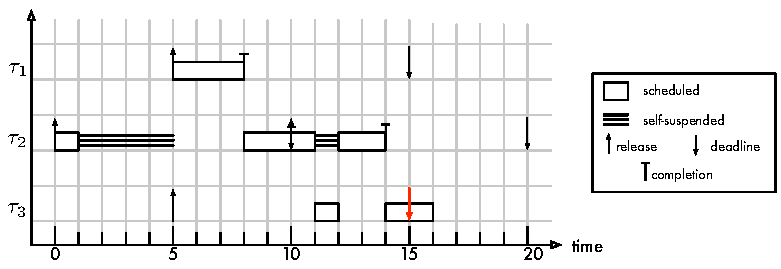
\includegraphics[scale=1]{../figures/not-ok-without-period-enforcer/not-ok.pdf}
  \caption{Example uniprocessor schedule (\emph{without} period enforcement) of three tasks $\tau_1 = $, $\tau_2$, and $\tau_3$ with periods $T_1 = T_2 = T_3 = 10$. Tasks $\tau_1$ and $\tau_3$ consist of a single computation segment ($C_1^1 = C_3^1 = 3$); task $\tau_2$ consists of two computation and one suspension segment ($C_2^1 = 1$, $S_2^1 = 4$, $C_2^2 = 2$). Jobs of tasks $\tau_1$ and $\tau_3$ are released just as $\tau_2$ resumes from its self-suspension at time~$5$. Without period enforcement, task $\tau_3$ misses a deadline at time~$15$ because the second job of  task $\tau_2$ suspends only briefly (for one time unit rather than four).}
  \label{fig:not-ok-without-period-enforcement}
\end{figure}


The key idea underlying the period enforcer algorithm is to artificially delay the execution of computation segments if a job resumes ``too soon.'' To this end,  the period enforcer algorithm determines for each computation segment an \emph{eligibility time}. If a segment resumes  before its eligibility time, the execution of the segment is delayed until the eligibility time is reached.

A segment's eligibility time is determined according to the following rule. Let $ET_{i,j}^k$ denote the eligibility time of the $k$\xth computation segment of the $j$\xth job of task $\tau_i$. Further, let $a^k_{i,j}$ denote the segment's arrival time. Finally, let $\mathit{busy}(\tau_i, t')$ denote the last time that a level-$i$ busy interval began on or prior to time $t'$ (i.e., the processor executes only $\tau_i$ or higher-priority tasks throughout the interval $[\mathit{busy}(\tau_i, t'), t']$). According to Section 3.1 in \cite{Raj:suspension1991}, the period enforcer algorithm defines the segment eligibility time of the $k$\xth segment as
\begin{align}\label{eq:ET-def}
	ET_{i,j}^k & = \max\left(ET_{i,j-1}^k + T_i,\ \mathit{busy}(\tau_i, a^k_{i,j})\right),
\end{align}
where $ET_{i,0}^k = -T_i$. 

Figure \ref{fig:ok-with-period-enforcement} illustrates how this definition of eligibility times restores the schedulability of the task set depicted in Figure~\ref{fig:not-ok-without-period-enforcement}. Consider the eligibility times of the second segment of task $\tau_2$.

By definition, we have $ET_{2,0}^2 = -T_2 = -10$. At time~5, when the second computation segment of the first job resumes ($a_{2,1}^2 = 5$), we thus have
\begin{align*}
	ET_{2,1}^2 & = \max\left(-T_2 + T_2,\ \mathit{busy}(\tau_2, a_{2,1}^2\right) ) = \max(0, 5) = 5
\end{align*}
since the arrival of $\tau_2$'s second segment (and the release of $\tau_1$) starts a new level-2 busy interval at time $a_{2,1}^2 = 5$. The second segment of $\tau_2$'s first job is hence immediately eligible to execute; however, due to the presence of a pending higher-priority job, $\tau_2$ is not actually scheduled until time~8 (just as without period enforcement as depicted in Figure \ref{fig:not-ok-without-period-enforcement}).

The second segment of the second job of $\tau_2$ arrives at time $a_{2,2}^2 = 12$. In this case, the segment is \emph{not} immediately eligible to execute since
\begin{align*}
	ET_{2,2}^2 & = \max\left(ET_{2,1}^2 + T_2,\ \mathit{busy}(\tau_2, a_{2,2}^2\right) ) = \max(5 + 10, 12) = 15.
\end{align*}
Hence, the execution of $\tau_2$'s second computation segment does not start until time $ET_{2,2}^2 = 15$, which gives $\tau_3$ sufficient time to finish before its deadline at time~$15$.


\begin{figure}[t]
  \centering
  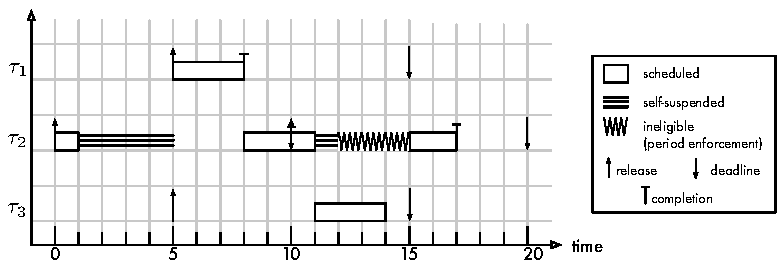
\includegraphics[scale=1]{../figures/ok-with-period-enforcer/ok.pdf}
  \caption{Example uniprocessor schedule \emph{with} period enforcement assuming the same scenario as depicted in Figure~\ref{fig:not-ok-without-period-enforcement}. With period enforcement, task $\tau_3$ does not miss a deadline because task $\tau_2$'s second computation segment is delayed until it no longer imposes undue interference (i.e., it is prevented from resuming ``too soon'').}
  \label{fig:ok-with-period-enforcement}
\end{figure}

The examples in Figures \ref{fig:not-ok-without-period-enforcement} and \ref{fig:ok-with-period-enforcement} suggest an intuition for the benefits provided by period enforcement: computation segments of a self-suspending task $\tau_i$ are forced to execute at least $T_i$ time units apart (hence the name), which ensures that it causes no more interference than a regular (non-self-suspending) sporadic task. Next, we revisit the original analysis of this technique.


\subsection{Classic Analysis of the Period Enforcer Algorithm}
\label{sec:classic-analysis}

The central notation in Rajkumar's analysis~\cite{Raj:suspension1991} is a \emph{deferrable task}, which matches our notion of segmented tasks.  Specifically, Rajkumar states that:
\begin{quote}
With deferred execution, a task $\tau_i$ can execute its $C_i$ units of execution in discrete amounts $C_i^1, C_i^2$, $\ldots$ with suspension in between $C_i^j$ and $C_i^{j+1}$. \cite[Section 3]{Raj:suspension1991}\footnote{The notation has been altered here for the sake of consistency. } 
\end{quote}

Note that it is not possible to convert a dynamic self-suspending task into the notion of deferred execution defined in \cite[Section 3]{Raj:suspension1991}, since the definition of a dynamic self-suspending task creates dynamic execution amounts for different jobs of a task. A simple example can explain why the period enforcer algorithm is not compatible with the dynamic self-suspending task model. Suppose that the system has only one task with execution time $C_1=1$, $S_1=1$, and $D_1=T_1=2$. The first job of task $\tau_1$ arrives at time $0$, suspends itself for one time unit, and then executes for one time unit. The second job of task $\tau_1$ arrives at time $2$, first executes for $0.5$ time unit, then suspends for $1$ time unit, and executes for $0.5$ time unit. With the period enforcer algorithm, the second job of task $\tau_1$ starts its execution at time $3$ and will clearly miss the deadline at time $4$.

%
Central to Rajkumar's analysis~\cite{Raj:suspension1991} is a \emph{task set transformation} that splits each deferrable task with multiple segments into a corresponding number of single-segment deferrable tasks.  In the words of Rajkumar~\cite[Section 3]{Raj:suspension1991}:

\begin{quote}
	 Without any loss of generality, we shall assume that a task $\tau_i$ can defer its entire execution time but not parts of it. That is, a task $\tau_i$ executes for $C_i$ units with no suspensions once it begins execution. Any task that does suspend after it executes for a while can be considered to be two or more tasks each with its own worst-case execution time. The only difference is that if a task $\tau_i$ is split into two tasks $\tau_i'$ followed by $\tau_i''$, then $\tau_i''$ has the same deadlines as $\tau_i{{'}}$. 
\end{quote}
%
In other words, the transformation can be understood as splitting each self-suspending task into a matching number of non-self-suspending sporadic tasks subject to release jitter, which can be easily analyzed with classic fixed-priority response-time analysis~\cite{ABRTW:93}. 

It is well known that uncontrolled deferred execution (i.e, release jitter) can impose  increased interference on lower-priority tasks because of the potential for ``back-to-back'' execution~\cite{LSS:87,LSST:91,Ra:90,ABRTW:93,SLS:95}, as illustrated in Figure \ref{fig:not-ok-without-period-enforcement}. 

The purpose of the period enforcer algorithm is to reduce such penalties for lower-priority tasks without detrimentally affecting the schedulability of self-suspending, higher-priority tasks. The latter aspect --- no detrimental effects for self-suspending tasks --- is captured concisely by Theorem 5 in the original analysis of the period enforcer algorithm \cite{Raj:suspension1991}.
\begin{quote}
{\bf Theorem 5}: A deferrable task that is schedulable under its worst-case conditions is also schedulable under the period enforcer algorithm.  \cite{Raj:suspension1991}
\end{quote}

\subsection{Questions Answered in This Paper}
\label{sec:questions}

Theorem 5 (in \cite{Raj:suspension1991}) is a strong result that seemingly enables a powerful analysis approach: if the corresponding transformed set of non-self-suspending tasks (subject to release jitter, without period enforcement) can be shown to be schedulable under fixed-priority scheduling using \emph{any} applicable analysis (e.g.,~\cite{ABRTW:93}), then the period enforcer algorithm also yields a correct schedule.

However, recall that, in the original analysis~\cite{Raj:suspension1991}, deferrable tasks are assumed to defer their  execution either completely or not at all (but not parts of it). It is hence important to realize that Theorem 5 in \cite{Raj:suspension1991} applies only to the \emph{transformed} task set---Theorem 5 in \cite{Raj:suspension1991} does \emph{not} apply to the \emph{original} set of segmented self-suspending tasks. This leads to the first question: \emph{Does schedulability of the transformed set of non-self-suspending tasks (subject to release jitter, without period enforcement) also imply schedulability of the original set of segmented self-suspending tasks (under period enforcement)?}  In Section \ref{sec:unschedulable}, we answer this question in the negative.

\begin{enumerate}
	\item There exist sporadic segmented self-suspending task sets that are schedulable under fixed-priority scheduling without any enforcement, but the corresponding schedule by using the period enforcer algorithm is not feasible. This shows that Theorem 5 in \cite{Raj:suspension1991} has to be  used with care --- it may be applied only in the context of the transformed single-segment deferrable task set, and not in the context of the original segmented self-suspending task set.
\end{enumerate}


Therefore, to apply Theorem 5 to conclude that a set of segmented self-suspending task sets remains schedulable despite period enforcement, we first have to answer the following question: \emph{Given a set of sporadic segmented self-suspending tasks, how do we obtain a corresponding set of (single-segment) deferrable tasks?} That is, the classic analysis of the period enforcer \cite{Raj:suspension1991} presumes that it is possible to convert self-suspension segments into equivalent bounds on release jitter, but it remains unclear \emph{how} this central step should be accomplished. In Section \ref{sec:convert}, we make a pertinent observation.

\begin{enumerate}
\setcounter{enumi}{1}
	\item Deriving a single-segment deferrable task set corresponding to a given set of sporadic segmented self-suspending tasks in polynomial time is an open problem. Recent findings by Nelissen et al.~\cite{ecrts15nelissen} can be applied, but their method takes exponential time.
\end{enumerate}

Finally, we make a third observation concerning the use of the period enforcer in conjunction with suspension-based multiprocessor locking protocols for partitioned fixed-priority scheduling (such as the MPCP~\cite{LNR:09,Ra:90} or the FMLP~\cite{BLBA:07,BA:08}). While it is certainly tempting to apply period enforcement with the intention of avoiding the negative effects of deferred execution due to lock contention (as previously suggested elsewhere~\cite{Raj:91,Lak:11,LNR:09}), we ask: \emph{Does existing blocking analysis remain safe when combined with the period enforcer algorithm?} In Section \ref{sec:locking}, we show that this is not the case.
\begin{enumerate}
\setcounter{enumi}{2}
	\item The period enforcer algorithm invalidates all existing blocking analyses as there exist non-trivial feedback cycles between the period enforcer rules and blocking durations.
\end{enumerate}



\section{Period Enforcement Can Induce Deadline Misses}
\label{sec:unschedulable}

In this section, we demonstrate with an example that there exist sporadic  segmented self-suspending task sets that both \textbf{(i)} are schedulable \emph{without} period enforcement and \textbf{(ii)} are not schedulable with period enforcement.

To this end, consider a task system consisting of $2$ tasks. Let $\tau_1$ denote a sporadic task without self-suspensions and parameters $C_1 = 2$ and $T_1=D_1=10$, and let $\tau_2$ denote a self-suspending task consisting of two segments with parameters  $C_2^1 = 1$,  $S_2^1 = 6$, $C_2^2=1$, and $ T_2=D_2=11$. Suppose that we use the rate-monotonic priority assignment, i.e., $\tau_1$ has higher priority than $\tau_2$. This task set is schedulable without any enforcement since at most one computation segment of a job of $\tau_2$ can be delayed by $\tau_1$: 
\begin{itemize}
	\item if the first segment of a job of $\tau_2$ is interfered with by $\tau_1$, then the second segment resumes at most after $9$ time units after the release of the job and the response time of task $\tau_2$ is hence $10$; otherwise,
	\item  if the first segment of a job of $\tau_2$ is not interfered with by $\tau_1$, then the second segment resumes at most $7$ time units after the release of the job and hence the  response time of task $\tau_2$ is at most $10$ even if the second segment is interfered with by $\tau_1$.
\end{itemize}
Figure \ref{fig:example-original} depicts an example schedule of the task set assuming periodic job arrivals.


\begin{figure}[t]
  \centering
  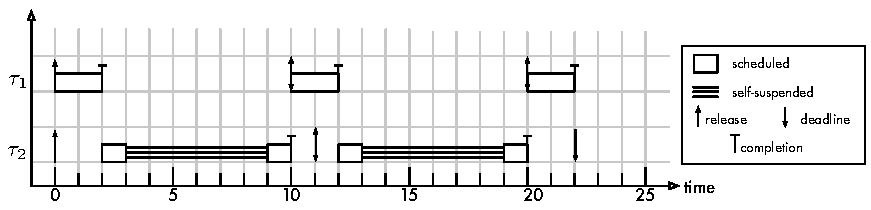
\includegraphics[scale=1]{../figures/example-original/example-original.pdf}
  \caption{An illustrative example of the original self-suspending task set (without period enforcement) assuming periodic job arrivals on a uniprocessor. Task $\tau_1$ has higher priority than task $\tau_2$.}
  \label{fig:example-original}
  \end{figure}
\begin{figure}[t]
  \centering
  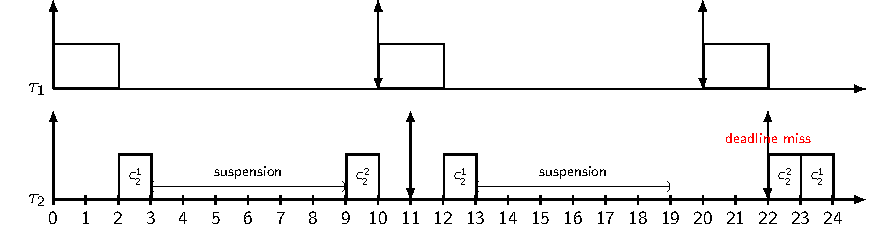
\includegraphics[scale=1]{../figures/example/example.pdf}
  \caption{An illustrative example demonstrating a deadline miss at time 22
    under the period enforcer algorithm. At time~19, $\tau_2$ resumes, but it remains ineligible to execute until time~20 when $\tau_1$ is released.}
\label{fig:example}  
\end{figure}


Next, let us consider the same task set under control of the period enforcer algorithm, as defined in Section \ref{sec:pe}.
Figure \ref{fig:example} shows the resulting schedule for a periodic release pattern. The first job of task $\tau_2$ (which arrives at time $a^1_{2,1} =  0$) is executed as if there is no period enforcement since the definition $ET_{2,0}^1 = ET_{2,0}^2 = -T_2$ ensures that both segments are immediately eligible. Note that the first segment of $\tau_2$'s first job is delayed due to interference from $\tau_1$. As a result, the second segment of $\tau_2$'s first job does not resume until time $a^2_{2,1} = 9$. Thus, we have
\begin{align*}
	ET_{2,1}^1 & = \max\left(-T_2 + T_2,\ \mathit{busy}(\tau_2, 0)\right) = 0  \text{ and }
\\
	ET_{2,1}^2 & = \max\left(-T_2 + T_2,\ \mathit{busy}(\tau_2, 9\right) ) = 9.
\end{align*}

In contrast to the first job, the second job of task $\tau_2$ (which is released at time $11$) is affected by period enforcement. The first segment of the second job arrives at time $a^1_{2,2} = 11$, is interfered for one time unit, and suspends at time $13$. The  second segment of the second job hence resumes only at time $a^2_{2,2} = 19$. Thus, we have
\begin{align*}
	ET_{2,2}^1 & = \max\left(0 + 11,\ \mathit{busy}(\tau_2, 11)\right) = 11  \text{ and }
\\
	ET_{2,2}^2 & = \max\left(9 + 11,\ \mathit{busy}(\tau_2, 19\right) ) = 20.
\end{align*}
According to the rules of the period enforcer algorithm, the processor therefore remains idle at time $19$ because the segment is not eligible to execute until time $ET_{2,2}^2 = 20$. However, at time $20$, the third job of $\tau_1$ is released. As a result, the second job of $\tau_2$ suffers from additional interference and misses its deadline at time $22$.




This example shows that there exist sporadic segmented self-suspending task sets that   \textbf{(i)} are schedulable under fixed-priority scheduling without any enforcement, but \textbf{(ii)} are not schedulable under the period enforcer algorithm.


One may consider to enrich the period enforcer with the following property: when the processor becomes idle, a task immediately becomes eligible to execute regardless of its eligibility time. However, even with this extension, the above example remains valid by introducing one additional lowest priority task $\tau_3$ with execution time $C_3=13$ (to be executed from time $3$ to time $9$ and time $13$ to time $20$) and $T_3=D_3=100$. With task $\tau_3$, the processor is always busy from time $0$ to time $23$ and consequently $\tau_2$ still misses its deadline at time $22$.



Furthermore, the example also demonstrates that the conversion to single-segment deferrable tasks does incur a loss of generality since it introduces pessimism. Recall that the analysis in Theorem 5 in~\cite{Raj:suspension1991} was only compatible with the deferrable task model. For the above example, we need to convert the segmented-suspending sporadic task $\tau_2$ into two deferrable tasks, called $\tau_2^1$ and $\tau_2^2$.
By converting the two computation segments of task $\tau_2$ into two deferrable tasks $\tau_2^1$ and $\tau_2^2$, we can conclude that  task $\tau_2^1$ never defers its execution and task $\tau_2^2$ defers its execution by at most \emph{$9$} time units.  Then the resulting single-segment deferrable task set $\{\tau_1, \tau_2^1, \tau_2^2\}$ is in fact not schedulable under the given fixed-priority scheduling since we can time the release of a job of $\tau_1$ to coincide with the arrival of a job of $\tau_2^2$ after it has maximally deferred its execution. We can easily see that the worst-case response time of the computation segment represented by task $\tau_2^2$ is $3$ time units after the second computation segment of task $\tau_2$ arrives. Together with the maximum deferred time $9$ time units, we know that the corresponding deferrable task set in fact has deadline misses since $9+3=12 > 11$. Therefore, the period enforcer algorithm may also cause a deadline miss.




%\clearpage
